It is already clearly established the presence of Bufferbloat at least three
networks, resulting in a decrease in the performance and usability of the
networks, resulting in catastrophic times of answer for anyone who wants to
have a smooth session with any other service that requires capacity of the
network.

Trying to assimilate otherwise these results is that in Figure
\ref{fig:smokenat} can see the contrast of the two opposite poles.

\begin{figure}
\begin{subfigure}{\textwidth}
  \centering
	%\rule{5.5cm}{7.1cm}
    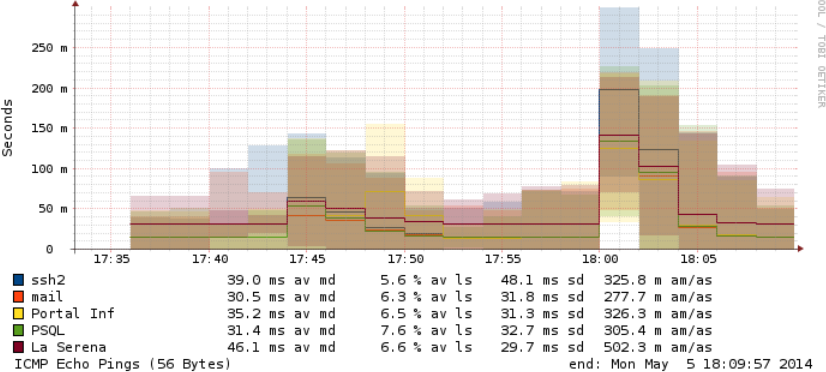
\includegraphics[width=0.8\textwidth]{img/smoke_nat_good}
\caption[Smokeping: Ping test to National servers with good performance]{Good performance Network}
\label{fig:smokenatgood}
\end{subfigure}%
\\
\begin{subfigure}{\textwidth}
\centering
	%\rule{5.5cm}{7.1cm}
    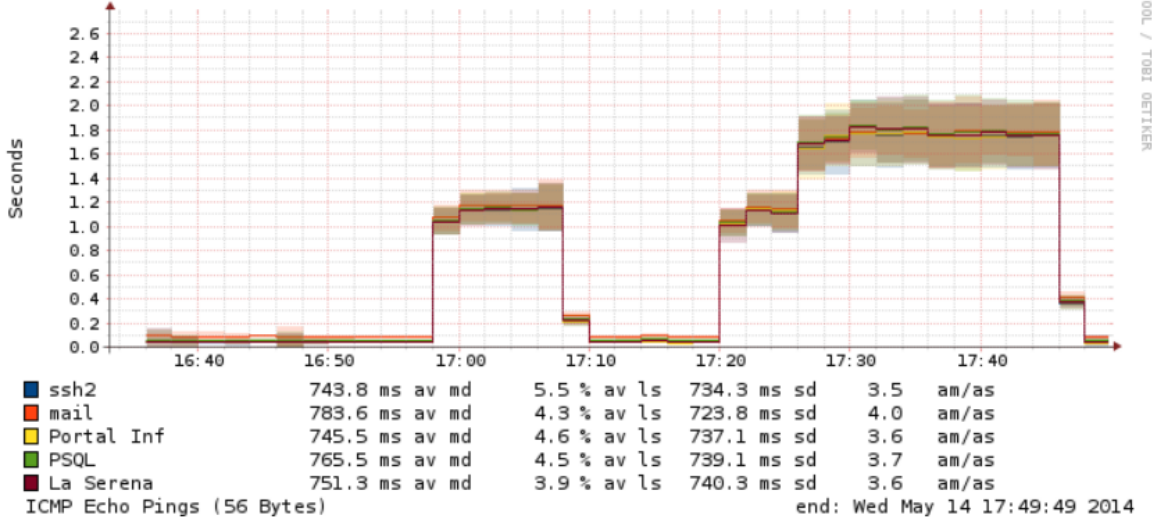
\includegraphics[width=0.8\textwidth]{img/smoke_nat_bad}
\caption[Smokeping: Ping test to National servers with bad performance]{Bad performance Network}
\label{fig:smokenatbad}
\end{subfigure}
\caption[Smokeping: Ping test to National servers]{Ping test to National servers}
\label{fig:smokenat}
\end{figure}

Figure \ref{fig:smokenatgood} shows the behavior of the network
\textit{casa\_w} which has faster response times with  no load around 50ms and
to superor  200ms with maximum use of the network. While can be appreciate
greater amount of \textit{``smoke''} (bar with same color as the line), this
is because by the time range that is driving (very low), tends generates this
small variation.

In contrast, in Figure \ref{fig:smokenatbad}, the amount of smoke is much
lower, but the variation in time is much higher, resulting in lower time to
100ms before loading, then vary drastically reaching over two seconds. While
this case was less packet loss, test took almost the double because of the
tendency to vary dramatically in the second case.


\begin{figure}
\begin{subfigure}{\textwidth}
\centering
	%\rule{5.5cm}{7.1cm}
    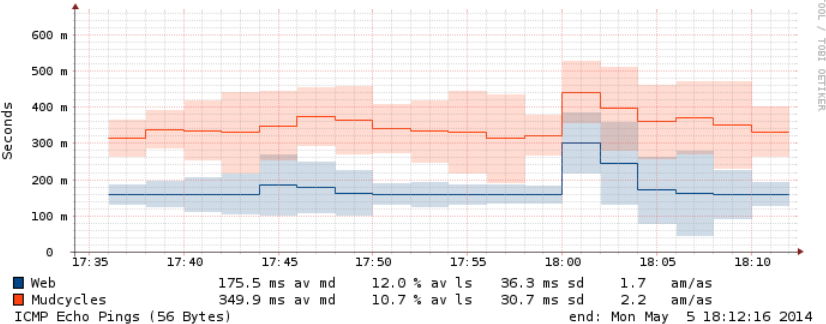
\includegraphics[width=0.8\textwidth]{img/smoke_int_good}
\caption[Smokeping: Ping test to International Servers with good performance]{Good performance network}
\label{fig:smokeintgood}
\end{subfigure}%
\\
\begin{subfigure}{\textwidth}
\centering
	%\rule{5.5cm}{7.1cm}
    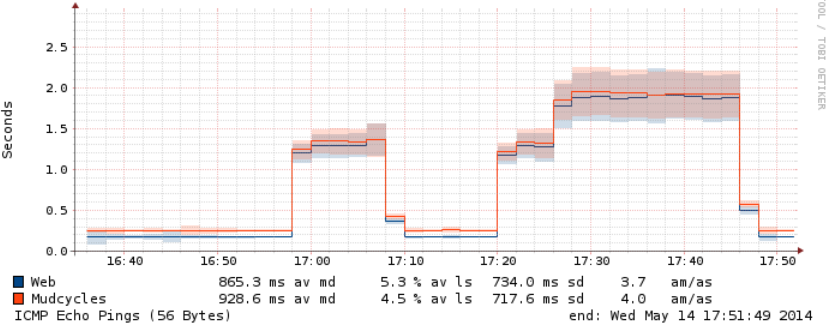
\includegraphics[width=0.8\textwidth]{img/smoke_int_bad}
\caption[Smokeping: Ping test to International servers with bad performance]{Bad performance network}
\label{fig:smokeintbad}
\end{subfigure}
\caption[Smokeping: Ping test to International servers]{Ping test to International servers}
\label{fig:smokeint}
\end{figure}

For international servers, it can be appreciated that the tendency remains
very strong. The times related to Figure \ref{fig:smokeintbad} increases to 8
times its minimum value, ranging from 250ms to about 2 seconds. Again, the
loss in Figure \ref{fig:smokeintgood} is almost double than in Figure
\ref{fig:smokeintbad}, but the latter spent a longer period without load,
which reflect that in average have lower loss.

It is also interesting to note that while both servers are in the U.S., the
requests to the server noticed by the orange line took almost twice the time
against the blue-line-host  (above 300ms). This may be due to the
characteristics of the service provided or the resolution time by the server
because after a little more investigation, it was determined that was hosted
on a VPS with characteristics similar to Iperf's server connection used (same
hosting service).

\begin{figure}
\begin{subfigure}{\textwidth}
\centering
	%\rule{5.5cm}{7.1cm}
    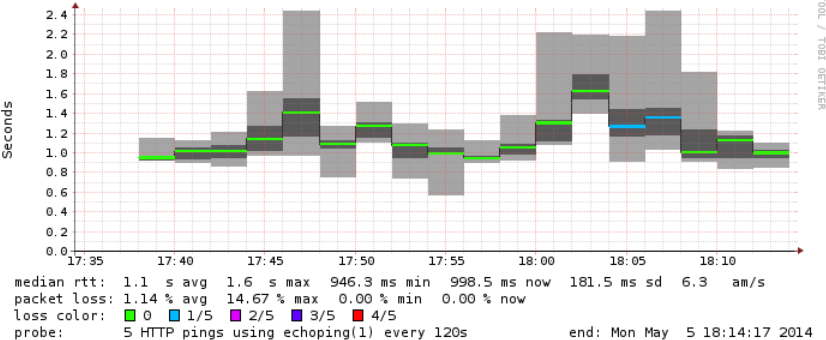
\includegraphics[width=0.8\textwidth]{img/smoke_inf_good}
\caption[Smokeping: Web requests with good performance]{Good performance network}
\label{fig:smokewebgood}
\end{subfigure}%
\\
\begin{subfigure}{\textwidth}
\centering
	%\rule{5.5cm}{7.1cm}
    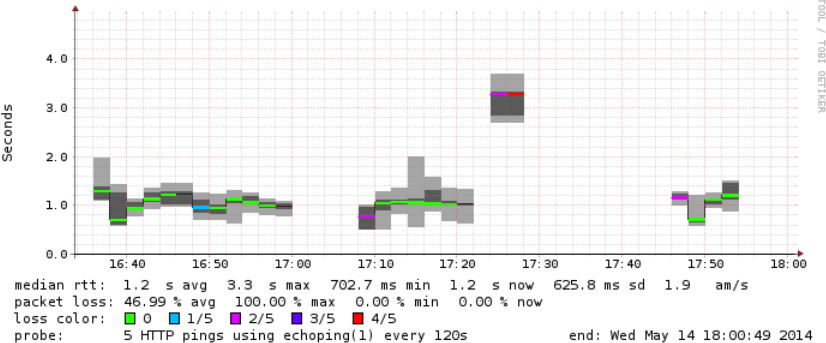
\includegraphics[width=0.8\textwidth]{img/smoke_inf_bad}
\caption[Smokeping: Web requests with bad performance]{Bad performance network}
\label{fig:smokewebbad}
\end{subfigure}
\caption[Smokeping: Web requests to National servers]{Web requests to National servers}
\label{fig:smokeweb}
\end{figure}

To conclude, Figure \ref{fig:smokeweb}  reveal the results of the HTTP
requests. In the case of Figure \ref{fig:smokewebgood}, load average achieved
was 1.1 seconds  with a loss of approximately 1.14\%. In contrast, in Figure
\ref{fig:smokewebbad}, right after the first overload (close at 17:00 hrs) of
the network, communication is affected, only been able to resume the
communication upon completion of the test. In the second iteration, becomes
not only intermittent communication, but also when it generate some traffic,
it takes about 3 seconds and has a loss of about 70\%. This not only affirms
our theory about the behavior and relationship to loss over time that lasted
the test, but also shows how terrible it would be for anyone trying to load
any website.
